\documentclass{article}
\title{CP-ALS-QR report}
\author{Alex Zhang}
\date{July 2023}
\textwidth=16.00cm 
\textheight=22.00cm 
\topmargin=0.00cm
\oddsidemargin=0.00cm 
\evensidemargin=0.00cm 
\headheight=0cm 
\headsep=0.5cm
\textheight=610pt
\usepackage{graphicx}
\usepackage{multicol}
\usepackage{tikz}


\graphicspath{ {./images/} }

\usepackage{latexsym,array,delarray,amsthm,amssymb,epsfig}
\usepackage{amsmath}
\usepackage{listings}
\lstset{
  basicstyle=\ttfamily,
  mathescape
}

\newcommand{\bmat}[1]{\begin{bmatrix} #1 \end{bmatrix}}
\newcommand{\mat}[1]{\mathbf{#1}}
\newcommand{\ten}[1]{\mathcal{#1}}
% matrix/vector/tensor/element macros
\usepackage{bm}
\newcommand{\Tra}{T}										% transpose
\newcommand{\M}[2][]{\bm{#1{\mathbf{\MakeUppercase{#2}}}}} 		% matrix
\newcommand{\Me}[3][]{\bm{#1{\mathbf{\MakeUppercase{#2}}}}({#3})} 		% matrix entry
\newcommand{\Mb}[3][]{\bm{#1{\mathbf{\MakeUppercase{#2}}}}_{#3}}       	% submatrix
\newcommand{\Mbe}[4][]{\bm{#1{\mathbf{\MakeUppercase{#2}}}}_{#3}({#4})}	% submatrix entry
\newcommand{\Ms}[3][]{\bm{#1{\mathbf{\MakeUppercase{#2}}}}^{(#3)}}       	% matrix in series
\newcommand{\Mbs}[4][]{\bm{#1{\mathbf{\MakeUppercase{#2}}}}_{#3}^{(#4)}}   % submatrix in series
\newcommand{\V}[2][]{\bm{#1{\mathbf{\MakeLowercase{#2}}}}} 		% vector
\newcommand{\Vs}[3][]{\bm{#1{\mathbf{\MakeLowercase{#2}}}}^{(#3)}} 		% vector in series
\newcommand{\Ve}[3][]{\bm{#1{\mathbf{\MakeLowercase{#2}}}}({#3})}		% vector entry
\newcommand{\T}[2][]{#1{\mathbf{\cal{#2}}}} 						% tensor
\newcommand{\Te}[3][]{#1{\mathbf{\cal{#2}}}({#3})}		

\let\ds\displaystyle

\begin{document}

\maketitle
\section{Introduction}
%The CANDECOMP/PARAFAC or canonical polyadic (CP) decomposition for multidimensional data, 
%or tensors, is a popular tool for analyzing and interpreting latent patterns that may be 
%present in multidimensional data. Basically CP decomposition of a tensor refers to its
%expression as a sum of $r$ rank-one components and each of them is a vector outer product.
%One of the most popular methods used to compute a CP decomposition is the alternating least
%squares (CP-ALS) approach, which solves a series of linear least squares problems. Usually
%to solve these linear leaste squares problems, normal equations are used for CP-ALS. This
%approach may be sensitive for ill-conditioned inputs. Based on this idea, there are already
%a more stable approach which is solving the linear least sqaures problems using QR decomposition
%instead.

%For my summer research project, I basically follows the QR apprach but trying to 
%improve the efficiency for QR decomposition when assuming the input tensor is in Kruskal structure,
%that is, a tensor stored as factor matrices and corresponding weights. By exploiting this structure, 
%we improve the computation efficiency by not forming Multi-TTM tensor.
%The problem left is when doing CP-ALS, QR-based methods is exponential in $N$, the number of modes.
%The normal equations approach is linear in $N$ for Kruskal tensor. During the summer I tried
%to revise and implement former QR method which archieved better stability than normal equations
%but computation time increases linearly with respect to $N$.


\section{Background}
\subsection*{CP Decomposition}
Given a $d$-way tensor $\T{X} \in \mathbb{R}^{n_1\times n_2\times \dots \times n_d}$, its
CP decomposition of rank $r \in \mathbb{N}$ can be represented as 
$$\T{X}(i_1,i_2,\dots, i_d) \approx \sum^{r}_{j=1}\mat{A_1}(i_1,j)\mat{A_2}(i_2,j) \dots \mat{A_r}(i_r,j)$$
$$\text{for all } (i_1,i_2,\dots, i_d) \in [n_1] \otimes [n_2] \otimes [n_3] \otimes \dots \otimes [n_d]$$
Where $\mat{A_k} \in \mathbb{R}^{n_k \times r}$ is a factor matrix for all $k \in [d]$. There is also one visualization
for CP Decomposition for a 3-way tensor in following Figure 1.
\begin{figure}[ht!]
\centering
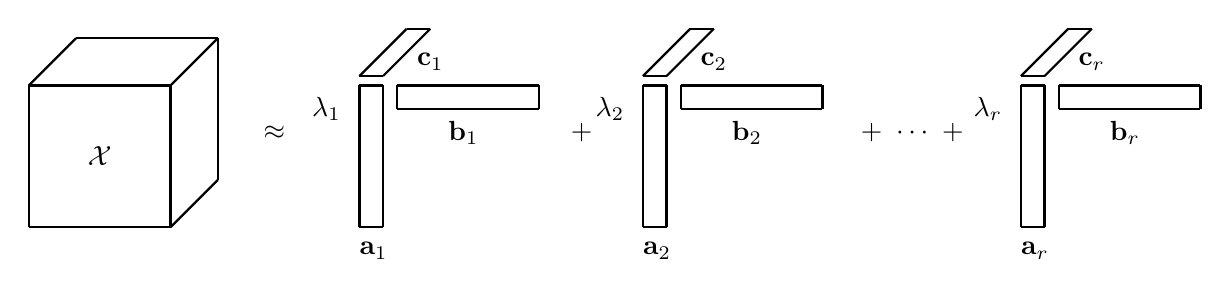
\begin{tikzpicture}[scale=0.6]
%\draw[step=1cm,gray,very thin] (0,0) grid (28,6); %grid lines

\draw node (X) at (1.5, 2.5) {$\T{X}$};
\draw[thick] (0,1) -- (3,1);
\draw[thick] (0,1) -- (0,4);
\draw[thick] (0,4) -- (3,4);
\draw[thick] (3,4) -- (3,1);
\draw[thick] (0,4) -- (1,5);
\draw[thick] (1,5) -- (4,5);
\draw[thick] (3,4) -- (4,5);
\draw[thick] (4,5) -- (4,2);
\draw[thick] (4,2) -- (3,1);

\draw node at (5.2, 3) {$\approx$};

\draw node at (6.3, 3.5) {$\lambda_1$};

\draw node at (7.3, 0.5) {$\V{a}_1$};
\draw[thick] (7,1) -- (7.5,1);
\draw[thick] (7,1) -- (7,4);
\draw[thick] (7,4) -- (7.5,4);
\draw[thick] (7.5,1) -- (7.5,4);

\draw node at (9.2, 3) {$\V{b}_1$};
\draw[thick] (7.8,3.5) -- (7.8,4);
\draw[thick] (7.8,3.5) -- (10.8,3.5);
\draw[thick] (7.8,4) -- (10.8,4);
\draw[thick] (10.8,4) -- (10.8,3.5);

\draw node at (8.5, 4.5) {$\V{c}_1$};
\draw[thick] (7,4.2) -- (7.5,4.2);
\draw[thick] (7,4.2) -- (8,5.2);
\draw[thick] (8,5.2) -- (8.5,5.2);
\draw[thick] (7.5,4.2) -- (8.5,5.2);

\draw node at (11.7, 3) {$+$};

\draw node at (12.3, 3.5) {$\lambda_2$};

\draw node at (13.3, 0.5) {$\V{a}_2$};
\draw[thick] (13,1) -- (13.5,1);
\draw[thick] (13,1) -- (13,4);
\draw[thick] (13,4) -- (13.5,4);
\draw[thick] (13.5,1) -- (13.5,4);

\draw node at (15.2, 3) {$\V{b}_2$};
\draw[thick] (13.8,3.5) -- (13.8,4);
\draw[thick] (13.8,3.5) -- (16.8,3.5);
\draw[thick] (13.8,4) -- (16.8,4);
\draw[thick] (16.8,4) -- (16.8,3.5);

\draw node at (14.5, 4.5) {$\V{c}_2$};
\draw[thick] (13,4.2) -- (13.5,4.2);
\draw[thick] (13,4.2) -- (14,5.2);
\draw[thick] (14,5.2) -- (14.5,5.2);
\draw[thick] (13.5,4.2) -- (14.5,5.2);

\draw node at (18.7, 3) {$+ \ \cdots \ +$};

\draw node at (20.3, 3.5) {$\lambda_r$};

\draw node at (21.3, 0.5) {$\V{a}_r$};
\draw[thick] (21,1) -- (21.5,1);
\draw[thick] (21,1) -- (21,4);
\draw[thick] (21,4) -- (21.5,4);
\draw[thick] (21.5,1) -- (21.5,4);

\draw node at (23.2, 3) {$\V{b}_r$};
\draw[thick] (21.8,3.5) -- (21.8,4);
\draw[thick] (21.8,3.5) -- (24.8,3.5);
\draw[thick] (21.8,4) -- (24.8,4);
\draw[thick] (24.8,4) -- (24.8,3.5);

\draw node at (22.5, 4.5) {$\V{c}_r$};
\draw[thick] (21,4.2) -- (21.5,4.2);
\draw[thick] (21,4.2) -- (22,5.2);
\draw[thick] (22,5.2) -- (22.5,5.2);
\draw[thick] (21.5,4.2) -- (22.5,5.2);
\end{tikzpicture}
\caption{CP decomposition of rank $R$ for a three-dimensional tensor $\T{X}$ \label{fig:3d-cp-decomp}}
\end{figure}
\subsection*{Linear Least Square Problem}
In mathmatical form, a sample least square problem is like 
$$\min_{\mat{X}}||\mat{B} - \mat{X}\mat{A}^\top||_{F}$$
Solving this least sqaure problem has several different techniques, Two most related methods for this report
is using Normal Equation and QR decomposition.
For normal equation, we take the gram of $\mat{A}$ and then compute $\mat{A}^\top\mat{B}^\top$. In sample equation we perform
\begin{align}
\mat{X}\mat{A}^\top\mat{A} &= \mat{B}\mat{A} \nonumber \\
\mat{A}^\top\mat{A}\mat{X}^\top &= \mat{A}^\top\mat{B}^\top \nonumber \\
\mat{X}^\top &= (\M{A}^\top\mat{A})^{-1}\mat{A}^\top\mat{B}^\top \nonumber
\end{align}
Which the time complexity for using normal equation will be $O(n^3)$, given $\mat{A} \in \mathbb{R}^{n \times n}$.

For QR factorization, we will first compute QR decomposition for matrix $\mat{A} = \mat{Q}\mat{R}$ and then apply inverse of $\mat{R}$. In term
of sample problem, we will do
\begin{align}
  \mat{X}\mat{A}^\top &= \mat{B} \nonumber \\
  \mat{X}(\mat{Q}\mat{R})^\top &= \mat{B} \nonumber \\
  \mat{X}\mat{R}^\top\mat{Q}^\top\mat{Q} &= \mat{B}\mat{Q} \nonumber \\
  \mat{X}^\top &= \mat{R}^{-\top}\mat{B}\mat{Q} \nonumber
\end{align} 
The time complexity for solving least square problem with QR factorization will be $O(n^3)$.

If speed is the only consideration, using normal equation will be better because of smaller coeffieicnt
for leading polynomial. However, this method will not always be stable with the presence of rounding error.
Because the condition number will increase when taking the gram of $\mat{A}$. Numberically speaking, solving least square through QR decomposition
is more preferred.





\subsection*{CP-ALS}
In terms of the work in CP-ALS, we need to solve least square problem in the form 
$$\min_{\mat{\hat{A}}_n}||\mat{X_{(n)}} - {\mat{\hat{A}_n}}\mat{Z}^\top_n ||$$
where $\mat{X_{(n)}}$ is the matricized tensors, $\mat{\hat{A}_n}$ is the factor matrix we are about to solve and 
$\mat{Z}^\top_n$ is transpose of the Khatri-Rao product of all factor matrices except $n$-mode which
$$\mat{Z}^\top_n = (\mat{A}_N \odot \mat{A}_{N-1} \odot \dots \odot \mat{A}_{n+1} \odot \mat{A}_{n-1} \odot \dots \odot \mat{A}_1)^\top $$ 


\subsection*{CP-Rounding}


\subsection*{CP-ALS-QR}
\subsubsection*{Dense}
\subsubsection*{Kruskal}
\subsubsection*{Complexity}




\section*{Result}
For showing the result, we setup an ill-conditioned problem which is sine of sums approximation problem.
In this test, we need to represent this N-dimensional function in a low rank linear representation instead of 
a exponential one. This problem can lead to ill-conditioned least sqaures problem in CP-ALS.

We first ran one linear least square test problem which takes this 6-way sin of sums Kruskal tensor as an input,
,tries to solve a least square problem on the last factor matrix, and compute the error between original full ktensor 
and the full ktensor that has been approximated. We did visualization for both runtime and accuracy showed in figure $1$.

\begin{figure}[ht!]
  \begin{center}
    \includegraphics*[scale = 0.4]{6way.jpg}
    \includegraphics*[scale = 0.4]{6way_acc.jpg}
    \caption[Figure]{runtime for pairwise Elim, normal equation, and explicit QR}
  \end{center}
here should have one error figure.
\end{figure}
Based on these two figures, we can know that new QR-based method will have roughly the same runtime
with normal equation but has better accuracy when solving least square problem.

In the next step, I put new QR-based method into CP-ALS technique which further compare the runtime and accuracy to 
CP-ALS using normal equation. There are also some visualization showed in Figure $3$.

\begin{figure}[ht!]
  \begin{center}
    \includegraphics*[scale = 0.3]{accuracy.jpeg}
    \includegraphics*[scale = 0.3]{runtime.jpeg}
    \caption[Figure]{runtime and accuracy figure for CP-ALS}
  \end{center}
add description
\end{figure}

As showed in Figure $3$,
the accuracy plot shows that CP-ALS can't achieve relative error much below the square root 
of machine precision, but CP-ALS-QR gets to around 1e-13. The yellow line indicates the difference
between input and the actual solution given by the formula. It is just a reference which we don't
expect both algorithms will get close to it.

The runtime plot indicates that both algorithms have time that depends linearly on n.  
They have different slopes, and in particular the slope of CP-ALS-QR is better, 
because CP-ALS does redundant computation for each subiteration while our implementation 
of CP-ALS-QR avoids this.  So the speedup increases with n (and will also increase with d).
Throughout the test, we used built-in CP-ALS function in tensor toolbox, which there are some redundant computation 
which can be improved.




\section*{Conclusion}










\end{document}